\chapter{State of the Art}
The State of the Art in NDN and Blockchain was thoroughly investigated when researching this project. This was done to establish what technologies are currently implemented in Named Data Networking and also to identify similar projects to our own solution.\par It is important to note this was done to a lesser extent for Blockchain because it is a supplemental technology in the Cryptocurrency space and is relatively simplistic(i.e. a vector of blocks all hashed with the previous block's hash).The Blockchain ``itself requires minimal structure"\cite{08}. Therefore, the different nuances of the technology which deviate from the fundamentals weren't investigated as thoroughly as it was beyond the scope of the project specification which asked for a proof of concept Blockchain. A `full fat' Blockchain solution involves miner nodes solving basic ``Proof-of-Work" or cryptographic puzzles\cite{09}, based on a timestamped transaction, appending them to a chain, and advertising that chain to all nodes in the network. 

This chapter is divided into Knowledge and Literary Review sections. The knowledge contextualizes this project by giving in depth background on all the technologies in use. 

The Literary Review then describes each individual paper from which this information was obtained. 

\section{Background and Summary}
In 2006, Van Jacobson likens the ICN solution for the IP problem to the Copernican solution for the Solar System problem.\cite{010} What he suggests by saying this is that IP was a(good) solution but for an entirely different problem than what the Internet is today. ``While it is entirely doable to predict the movement of planetary bodies by taking the Earth to be the center of the universe, it is incredibly complex. This is because the point-of-view is wrong." \cite{011} 
\\
In a similar way, despite the plethora of problems that IP was able to address at the turn of the last century - in today's world it causes more problems than it solves. This is because the IP abstraction's benefits no longer outweigh the drawbacks. In fact, in order for one to even connect to the Internet, we need to break the IP abstraction and do a complicated Dynamic Host Configuration Protocol dance which dictates that in order for us to gain access to a website, we must first gain an IP, which we must ask for, of a DHCP, which will be given to us once we ask an Address Resolution Protocol server, to send our MAC to a DHCP server, which can then give us an IP, which we can then use to ask for the nearest DNS server to respond to our request for a website IP. 
\\
NDN does away with all of this by just having nodes broadcast the Names of the data they want in an Interest packet. It is a completely different way to think about Networking, because the network participants or nodes no longer care where the Data is going. \par 
\begin{itemize}

\item Telephony concerns itself with having a direct end-to-end path in order to establish communication.
\item IP concerns itself with having a connected graph and a destination address
\item NDN doesn't concern itself with having a destination for a particular request but rather just propagating that request through the network.
\end{itemize}
Dissemination Networking is what Van Jacobson Proposes. Ask for Data - not an IP address. The background for this research splits off into two parts. The Blockchain technology is largely based on cryptography and hashing. NDN on the other hand has its roots in networking. 

\section{State of The Art - Knowledge}
This section will give a brief overview of how these two technologies - Blockchain and NDN, and their components, work.\par 
The paper splits the Knowledge section into a Blockchain description, followed by an overview of NDN and all of its main components.
\subsection{Blockchain}
A Blockchain is a distributed ledger of immutable digital records\cite{012}. It was conceptualized in a paper called ``Bitcoin - A Peer to Peer Electronic Cash System". The paper was written by Satoshi Nakamoto, an enigma of the cryptology world, who has even been speculated to be one of Trinity's own graduate crypto students - Michael Clear. The Blockchain is the main component of the Bitcoin cryptocurrency. It allows for decentralized transactions by solving the Byzantine Generals Problem\cite{013}. This is also known as having Byzantine Fault Tolerance(BFT). The Byzantine Generals Problem was first theorized about in a paper by the same name, authored by Leslie Lamport, Robert Shostak, and Marshall Pease in 1982. \par 
The Byzantine Generals Problem proposes a situation where a number of Generals from Byzantium have laid siege on an enemy city. The events of the problem develop somewhere in the Byzantine Empire, 1000 years ago. \par
Each General has an army. The problem they are faced with is taking an enemy city. Each of the Generals commands their own army. The Generals are aware that they can only take the city if they all order all of their respective armies to attack together in a \textbf{coordinated effort}. However, no General will commit to the attack without assurance that the others will also commit. In order to commit to an attack, the Generals must agree on a battle plan and a time of attack. There are a couple of problems with this:
\begin{itemize}
\item The messengers could be captured
\item The Generals would need to reply with confirmations
\item The Generals can change their minds, or be traitors and lie
\end{itemize}
The problem is that even if they agree on a time, no General can ever be sure that the others will attack with him because \textbf{confirmations are not instant.} This means that by the time a messenger arrives at General A's camp declaring General B's confirmation for an attack at a certain time, General B could've changed their mind and could've sent another messenger to relay the new message. This renders the original messenger's declaration invalid but General A doesn't know that. This cycle continues and the Generals can never be 100\% certain when to attack because they can never know what the other Generals are thinking in that instant of time.

The Blockchain addresses the inability of traditional systems, without a central authority, to determine that a certain resource hasn't been spent more than once. The reason banks or ``central authorities" can vouch for transactions, and guarantee against double spending, is because the transactions don't happen instantaneously. They are each, individually confirmed, and also, should the bank make a mistake, it covers it(insurance).\par 
The reason this isn't the case in a Blockchain distributed ledger system like Bitcoin, is because miners do Proof-of-Work in a peer-to-peer network. The network timestamps each transaction, making them secure by hashing them into a hash-based proof-of-work. The resulting record cannot be altered without redoing this proof-of-work. This consensus mechanism\cite{014} mirrors a voting system. There is a network, where nodes must know if an operation is valid. In order to do this, the nodes pool their CPU resources to do proof-of-work on transactions nodes accept to be valid, in order to verify them. If a transaction does not get their vote of confidence, they don't work on hashing that into the Blockchain. If the majority of nodes in the system are ``good", then the largest Blockchain generated will be valid.
\begin{figure}[ht] 
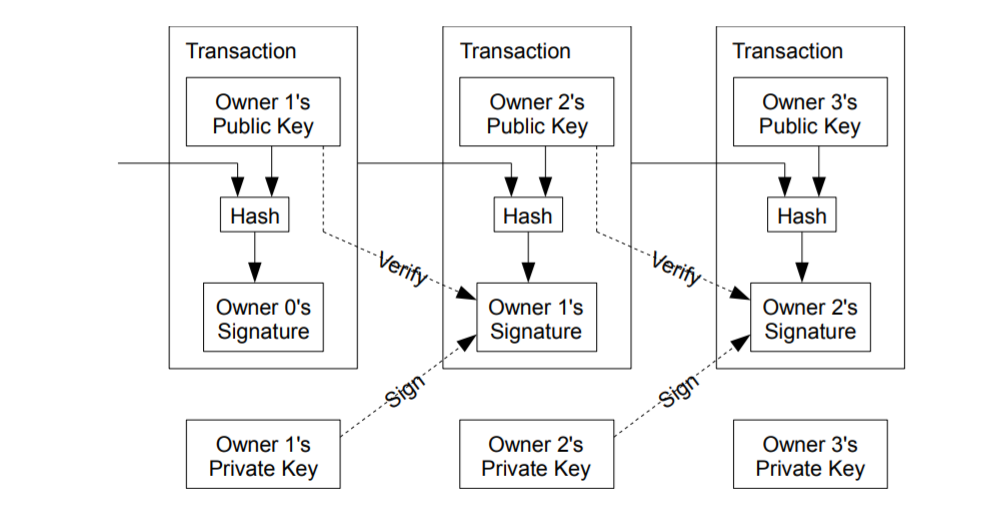
\includegraphics[width=6in]{hashes.png}
\caption{Blockchain structure\cite{015}}
\end{figure}

\subsection{NDN}
Named Data Networking began life in 2010 under the NSF's Future Internet Architecture\cite{016}. The leading effort in the NDN project has been UCLA Professor Lixia Zhang. Projects like NDN picked up traction after CCN began development at PARC, headed by Van Jacobson. NDN presents a paradigm shift for the Networking Stack. Instead of IP being the thin-waist of the stack, NDN suggests a data name abstraction, where the name of the content becomes this thin-waist. \par
NDN is composed of a number of modules described below. It is a name based architecture where nodes in a network can request data, not based on where it comes from but based on the name of the data. E.g.: a node requests \textbf{/ndn/a-site/important/information} instead of an IP address. This abstraction is hugely advantageous in today's Internet where content sharing is at the forefront of what the Internet delivers. NDN allows for nodes to respond to Interests, which are content requests, with Data packets which are the content. Nodes interact by sending Interests by Name. Data is retrieved in Data packets.\par 
\begin{figure}[h]
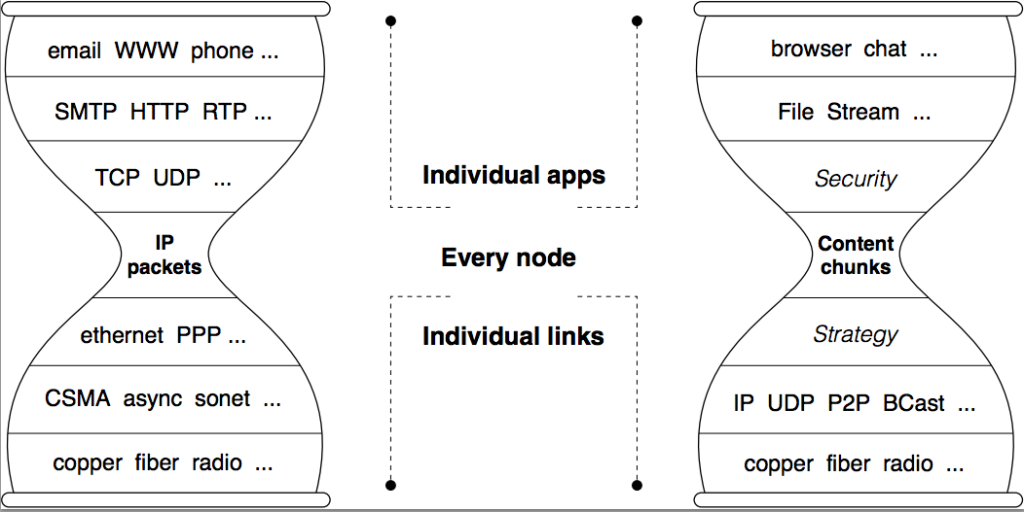
\includegraphics[width=6in]{hourglass.png}
\caption{The Networking Stack\cite{017}}
\end{figure}
\subsection{Names}
An NDN Name is a hierarchical name for NDN content, which contains a sequence of name components.\cite{018} Each NDN name component  consists of variable lengths and is separated by a `/' separator. This design is advantageous because it is human readable and allows for users to configure Interest and Data filters using regular expressions. \\
E.g: InterestFilter$(^<ndn><lectures>)$ means listen for any interests beginning with /ndn/lectures. 
Named Data Networking is all about names. When presenting on NDN at MILCOM 2017 in Baltimore, Lixia Zhang said ``the secret to NDN is in the names!" This is because this networking paradigm  is entirely centered on the names of content. Each entity in a network has an identity, and each identity has a name. Each named entity in a network follows a hierarchical naming scheme.\par
Names are represented by the name class in NDN. They are made up by a URI string. In C++, they are defined using the C-style const char* array. \par
Packets are forwarded using Longest Name Prefix Matching(LNPM)\cite{019}. 

It is similar to IP Longest Prefix Match where a routing algorithm will, upon needing to do a look-up, return the longest matching address. E.g:
Consider the following IPv4 Forwarding Table(CIDR Notation):\\
\begin{figure}[ht]
\centering
\begin{tabular}{|c|}
\hline
192.168.20.16/28\\
\hline
192.168.0.0/16\\
\hline
\end{tabular}
\caption{Forwarding Table}
\end{figure}

If the router was to look-up 192.168.20.19, both entries will ``match", but the router will only return 192.168.20.16/28 since the submask /28 is longer than the other entry's /16 submask\cite{020}.

A similar example could be given an Interest arriving at node B asking for \textbf{/ndn/a-site/lectures/telecomms/slides}  and node B's FIB could have entries for \textbf{/ndn/a-site} and \textbf{/ndn/a-site/lectures/telecomms/} in which case it will only return the second entry. \par 

The problem with LNPM comes from the inherent differences between address lengths in IP and NDN. In most cases, NDN names will be longer than IP as the namespace is unbounded. The difference in size is so drastic, that TCAM or SRAM memory modules for the FIB would not be large enough if the number of rules is large. The NDN FIB has to use DRAM in order to accommodate for this size difference. With such a difference in size and complexity, look-ups can take O(k) string look-ups\cite{021}.\par 
This is why NDN employs two techniques proposed in a Washington University paper by Haowei Yuan and Patrick Crowley. The first changes the LNPM design to a binary search of hash tables reducing lookups to O(log(k)) for prefixes with k components \cite{022} and the second technique is level pulling to improve the average case. This makes the name prefix lookup solution scalable - a necessary feature for the NDN architecture to work. 

\subsection{Faces}
Faces are abstractions of physical and virtual interfaces\cite{023}. They provide the main methods for NDN communcation. Faces hold a connection to a forwarder and support Interest/Data exchanges\cite{024}.In order to communicate in an NDN network, each entity must have a Face. Because Faces abstract away physical and virtual interfaces, it allows NDN to be used as an overlay network over existing technologies like IP\cite{025}
\begin{figure}[ht]
\centering
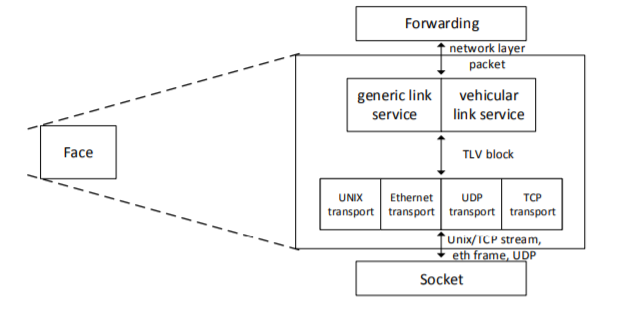
\includegraphics[scale=0.5]{facearch.png}
\caption{Face Architecture\cite{026}}
\end{figure}
\subsection{Interests}
An Interest is a data packet. It is integral to the design of NDN. Interest packets are sent out when nodes require data. If a node wants a piece of information it will send out an Interest with the Name of the data it requires. That Interest is then propagated through the nodes in the network. When the Interest arrives at another node, the node checks its Content Store for a signed piece of Data with a Name matching that of the Interest's. If no Data is found in the Content Store, the node stores the Face on which the Interest arrived in its Pending Interest Table(PIT), and appends it to a list of other Faces that have requested the same Data. It then checks its Forwarding Information Base(FIB). If it has information on which node might have the Data the first node required, it will forward that Interest on to that node, if not it will discard the interest. If that node then ever comes across that data it will check its PIT and if the Interests are still "fresh", it will forward the Data packet to all of the Faces that have expressed an Interest for the Data. It will then store the Data in its content store and discard all entries in its PIT. \par 
There are also Signed Interests, which used to be called Controller Interests. These Interests were designed because of the inherent inability of NDN nodes to send Data to each other without being prompted. This is why nodes can send Signed Interests which can request for another node to send and Interest for Data that the original node might have.
\begin{figure}[h]
\centering
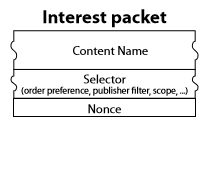
\includegraphics{interestpacket.png}
\caption{An Interest Packet\cite{027}}
\end{figure}
\subsection{Data}
Data packets are the other integral packets to the NDN design. Data packets are sent out when there is an Interest for them. They contain a X.509 Certificate which signs each Data packet. They also have a freshness value and obviously also contain bits of data.
\begin{figure}[h]
\centering
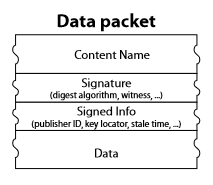
\includegraphics{datapacket.png}
\caption{A Data Packet\cite{028}}
\end{figure}
\subsection{Named-Data Forwarding Daemon}
Named-Data Forwarding Daemon(NFD) is responsible for handling all packets in the network. An instance of NFD runs on every node in a network. When a packet arrives on a Face, the NFD checks if that packet is destined for the particular node and if not it discards it based on a policy to allow/disallow unsolicited Data packets.
NFD is made up of the following modules: Core, Faces, Tables, Forwarding, Management, and Routing Information Base(RIB) Management.
\begin{figure}[ht]
\centering
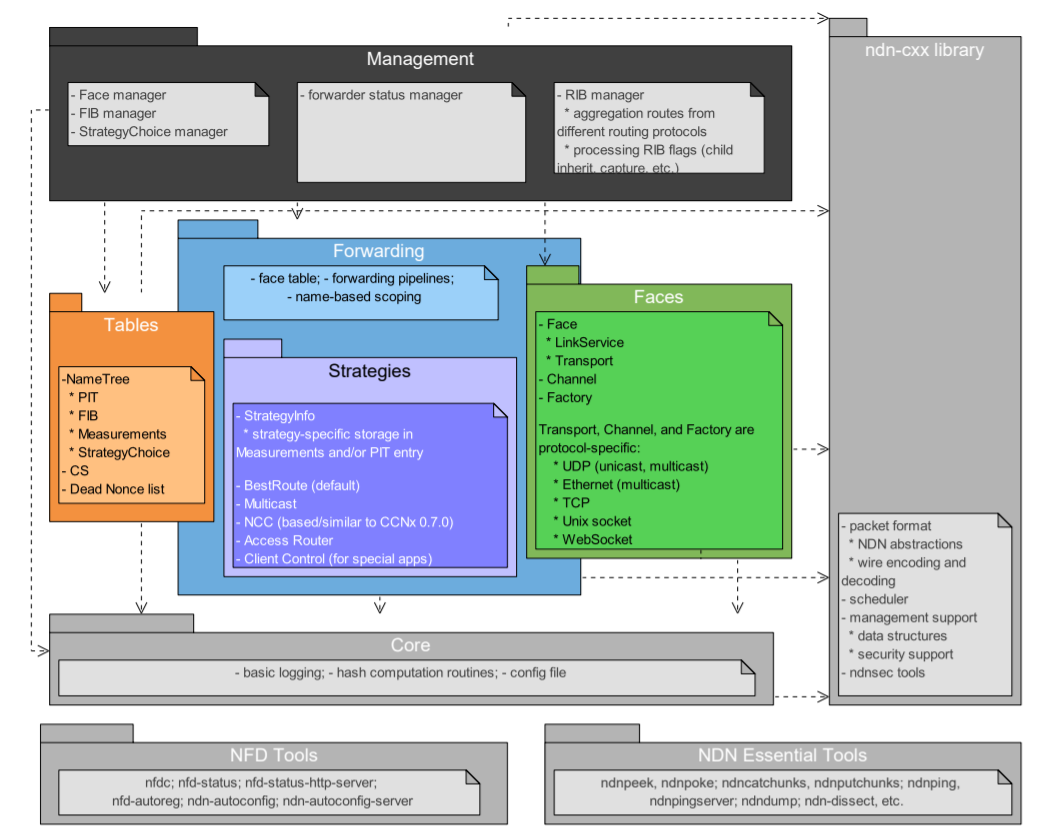
\includegraphics[scale=0.5]{nfd.png}
\caption{NFD Structure and Components[29]}
\end{figure}

\begin{itemize}
\item Core - Provide common services shared between modules like hash computation routines, DNS resolver, config file, face monitoring, etc.. \cite{029}
\item Faces - the NFD implements the Face abstraction
\item Tables - There are a number of tables that NFD is in charge of like the Content Store(CS), the Pending Interest Table(PIT) and the Forwarding Information Base(FIB).
\item Management - Implements the NFD Protocol, allowing applications to configure NFD.
\item RIB Management - The Routing Information Base is responsible for producing a consistent FIB, which is a non-trivial task because of the amount of ways it can be updated such as through different routing protocols, command line, application's prefix registration, etc.. The RIB is a module on its own, however it is managed by NFD.
\end{itemize}

\subsection{Named-Data Link State Routing}
Named-Data Link State Routing(NLSR) is the NDN module which deals with routing when a topology is created. It reuses an already established routing algorithm - link state. Its basic functionality is to discover adjacencies and disseminate both connectivity and name prefix information\cite{030}. NLSR works by sending out  Link State Advertisements(LSA) when a network is created to collect reachability and connectivity\cite{031} information. This means that each node has its Forwarding Interest Base populated with adjacent node names. NLSR takes time to converge proportional to CPU power in the Network. \par
There are two types of LSAs - \textit{named} and \textit{adjacency}. A name LSA will contain all the local prefixes registered locally with NLSR\cite{032}. An adjacency LSA contains all active links of a router and is updated by an active ChronoSync module which updates active routes when NLSR sends `hello' messages. If they time out three times, the connection has died and the adjacency LSA is updated. Whenever this LSA is updated for a router, the router advertises the new adjacency LSA to every node in the network. The latest versions of all adjacency LSAs are stored in the Link-State Database(LSDB).
\begin{figure}[ht]
\centering
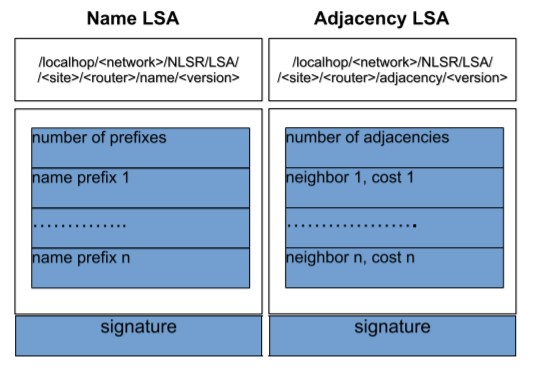
\includegraphics[scale=1]{lsa.png}
\caption{Link-State Advertisements\cite{033}}
\end{figure}
NDN can use the same routing algorithms that are used in IP such as Link-State and distance vectoring. There is one difference however, in the routing implementation for NDN. Whichever the implementation, routing must be able to offer multiple next hops(multipath) for nodes in the network, towards producers of Data. Fundamentally, the routing protocols are the same, with the exception that the Named-Data protocol must offer multipath.\par

NLSR offers a number of features, beneficial and crucial to NDN.
\begin{itemize}
\item Naming - NLSR uses hierarchically structured names to identify routers, routing processes, routing data and keys\cite{034}. 
\item Security - This feature comes as a by-product of the fact that each NLSR message is carried in an NDN Data packet which must be signed. 
\item Multi-Path - The main NLSR feature is multipath. While IP relies either on a single hop or limits its forwarding to multiple equal cost paths\cite{035} in order to avoid loops - this is not an issue in NDN. While the architecture doesn't encourage forwarding loops, they aren't a big concern because the NDN architecture simply allows, when forwarding, for each node to make a decision on where to send a packet. This is what is implemented in NDN's loop detection. 
\end{itemize}
\subsection{Chronosync}
Chronosync is a module used when there is a need for nodes to receive data or be updated at the same time. It is a vital module in networking configurations that run text messaging, group file sharing, screen-sharing, etc.. Chronosync runs on top of NFD and synchronizes Data and Interest packet sending and receiving. The Chronosync design splits into two parts: It maintains the state of a dataset, and it also has a logic module that responds to change\cite{036}. Chronosync monitors datasets and discovers state changes. However, it doesn't alter the dataset - this is left to the application layer. 
\begin{figure}[ht]
\centering
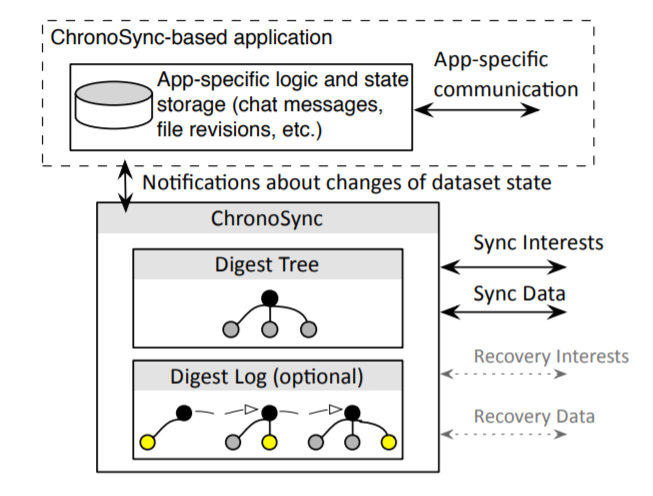
\includegraphics[scale=0.5]{chronosync.png}
\caption{Chronosync Overview \cite{037}}
\end{figure}
\subsection{Content Store}
The Content Store or cache is each node's local storage. It contains signed Data which the node can forward to any node expressing an interest for it. Caching is one of NDN's main features. There are two types - off path and on path caching. Off path caching, like the name suggests, disregards content path and just aims to replicate the content in a network\cite{038}. On Path caching is limited to the content propagated along the delivery path\cite{039} meaning the data cannot be cached outside the route from the node expressing the Interest for the Data and the producer of said Interest.
\subsubsection{Policies}
A number of policies exist for caching:FIX(0.9), DC and ProbeCache. A recent solution - ProbPD investigates content popularity as a heuristic for caching. All of the high-end solutions perform near identically.
\subsection{Security}
Ralph Merkle describes the problem with the classic\cite{040} Authenticated Public Key Distribution protocol. He describes how each node in a network generates a public key and stores it in a file system. If two nodes wish to agree on a common key in order to interact, they look up the Public Key portion of the other node. Then each send a \textbf{session key} encrypted with the other node's public key. Once in agreement, this key is secret and authenticated and can be used by both nodes to communicate. 

The problem with this approach is that a centralized file system is a single point of failure and is prone to attack. The attacks can be one of two - the public key elements can be altered in the file system(e.g. the attacking node could set another node's public key to be its own), and secondly, the private keys can be lost.

 The alternative to this approach is implemented in NDN and it is to introduce Certificates and a Certificate Authority(CA). Certificates refer to the binding of a node's keys to its identity i.e. which key belongs to which node. It is very important that there is a robust method of determining this key-identity bond and perhaps even more importantly, to ensure that it is immutable. ``In NDN, every entity that produces data needs to obtain an NDN certificate to prove the ownership of its namespace and cryptographic materials(public key)"\cite{041}.
 The security process occurs as following: First, we start off with the Achilles Heel for any networking security protocol - \textbf{bootstrapping}. This is the process of obtaining all trust anchors and certificates. 
	 
 Before that however, we need to just quickly define trust anchors(policies). They refer to the rules set by each entity to only accept packets of a desired format of names and name relationships\cite{042}. It is also important to note that these rules are governed by each identity at the Application Layer.
 
  Back to bootstrapping: In order to do this, nodes must obtain a namespace and then a certificate for that namespace from a CA that they trust\cite{043}. The order for entities receiving certificates is hierarchical. This means that if a user(entity) has obtained a certificate, it can delegate certificates to other entities within its namespace.
 Because trust anchors are determined at the Application Layer - the only prerequisite\cite{044} for security bootstrapping is allocating names. As long as an entity has a name, it can receive a certificate if allowed by the owner of the namespace. 
 Each entity has its own trust anchors but should naturally trust the Certificate Authority. In the case of the root namespace - that is the recognized CA by the root user, as for the rest of the names in the namespace, that is the root namespace.\par
 \textbf{NDNCERT} is a library found in NDN-CXX which provides the tools necessary for a name to obtain a certificate in an NDN network. It generates certificates for trust anchors automatically and manages them in a daemon\cite{045}. It runs in an instance called an agent and maintains all certificates generated by NDNCERT.\par
As well as that NDNCERT can revoke certificates automatically if they are considered unfit. There is a check done on each certificate and if it is generated illegally, then in the case of the MiniNDN emulator, the code will throw an error and exit the session.\par
Data packets are signed at creation time\cite{046}. This design choice is critical in the integrity of data packets in NDN because this means that a data packet physically cannot be sent off without being signed. The important bit here isn't so much that all data sent is signed as much as is the inverse - that all data received can be checked for a signature. 

This makes Data verification twofold: Firstly, NDN uses Trust Anchors - so if a node is expecting data, it can define a trust anchor that states that the data can only arrive from one particular \textbf{name}. Secondly, and this is the traditional, cryptographic verification method, once the Data packet is received and passes the trust anchor check, the consumer of the Data packet retrieves the corresponding certificate for the producer which is identified by the key name section in the packet\cite{047}. The Certificate will then recursively point to the root certificate and if all certificates along the way are valid that means that the Data packet itself is signed with a valid signature.

\section{Related Work}
There are a number of papers that I've come across that deal with security in NDN. As expected, there is plenty of work done in this field because it is a major concern for any network architecture.\par 

The NDN guides were a big help when it came to researching security. Spyridon Mastorakis' paper on NDN Security Support outlines all major features found in the Security module of NDN. This paper cited the Merkle paper on Public Key Distrtibution with Tree Authentication which is what is currently used in NDN.\par



However, when it came to Blockchain integration in NDN, there wasn't much work done in the field. Hashing, on one hand, is a big part of NDN security because of the size of NDN Names as described above. To this degree, much of Ralph Merkle's work has been employed in NDN, but the Blockchain concept in general isn't seen much. 

There is one particular paper titled BlockNDN by Kai Lei which describes a Blockchain abstraction for use in NDN in order to circumvent the IP architecture problem of lacking multicast support. This paper investigated whether Blockchain is a good fit for NDN. It outlined that the native support for multicast in NDN is a good starting point for the peer-to-peer Blockchain architecture and although it did not present a security solution involving Blockchain, this investigation was very useful when designing the solution for this paper. In BlockNDN, the concept of sync interests is introduced, where a node absent from the network would request a sync interest as opposed to request every single block in the chain individually. This paper goes into great detail of the entire process of creating blocks and publishing them. The BlockNDN project takes an interesting approach to broadcasting the information. Because of the nature of the Blockchain, Chronosync is not used to maintain a digest tree in order to maintain the system state. This is why, when a miner generates a node, it can simply send an interest with the node's hash value. \par

Another related solution which I used for some of its ideas was Alexander Afanasyev's paper titled NDNDelorean. This paper introduced a version concept for old data that needed to be authenticated. The version concept is quite useful when it comes to certificates. Because certificates can become invalid, it is important to be able to represent that in the Public Interest Base(PIB) and also the Blockchain. The problem with the Blockchain approach is that once appended to the Blockchain, a certificate can never be deleted without altering the whole Blockchain, which would render it invalid. This is why, instead we introduce ``version control" which in this project's case involves a simple integer(which could also be a boolean) which keeps track of a block's certificate's version. The current version is 1 if valid and 0 if invalid.
\section{Literary Review}
This section has been divided in the different technical components that have been investigated as part of this Final Year Project. Apart from being split into \textbf{NDN} and \textbf{Blockchain}, I've also split NDN into: \textbf{Security, NFD, NLSR, Mini-NDN, Content Store}.

The following table aims to quantify the usefulness of each paper that has been looked at. This method has been directly inspired by Masters student Conor Mooney who did an excellent job at scoring and qualifying his papers while researching. The categories for each paper reviewed fall under one of three categories: analysis, implementation, review.\\
\begin{itemize}
\item Analysis - Refers to papers which analyse a technology\\
\item Implementation - Refers to papers which discuss technical aspects of the technologies which were used. These papers were mostly the NDN Developer Guides.\\
\item Review - Reviews classify papers which mainly contribute with an evaluation - useful when there are different technologies that one might use for a particular problem, allowing for the narrowing down of solutions.\\
All papers will be scored based on a retroactive relevancy heuristic i.e. how useful did these papers end up being to the problems presented in this project. 
\end{itemize}
\begin{table} [!htb]
\centering
\begin{tabular}{l|c|c}
Paper & Type & Score \\ \hline
V. Jacobson - Networking Named Content & Analysis & 5\\
D. Kim - Efficient and Secure NDN & Implementation & 5\\
S. Weber - Caching & Implementation & 3\\
K. Lei - Blockchain Based Key Management & Implementation & 5\\
L. Zhang - Named Data Networking & Review & 4\\
S.Nakamoto - Bitcoin & Implementation & 4 \\
L. Zhang - NDN & Implementation & 4 \\
K. Huang - Cyber Attack Business & Review & 3 \\  
K. Lei - BlockNDN & Implementation & 5 \\ 
L. Wang - A Secure Link State Routing Protocol for NDN & Implementation & 5 \\ 
NFD Team - NFD Developer's Guide & Implementation & 4 \\ 
A. Afanasyev - NDN Technical Report 9 & Implementation & 4 \\ 
Y. Yu - NDN Delorean & Implementation & 4\\
S. Mastorakis - Security Support in NDN & Implementation & 5\\
W. Diffie \& M. Hellman - Privacy and Authentication & Implementation & 3 \\
R. Merkle - Protocols for PK Cryptosystems & Review & 3 \\
L. Kohnfelder - Central Authority & Implementation & 3  \\
B. Rainer \& S. Petscharing - NDN In V2E&Review&4\\
A. Afanasyev \& Z. Zhu - Let's Chronosync & Implementation & 3 
\end{tabular}
\caption{Relevancy of Papers}

\end{table}
\subsection{NDN}
\subsubsection{Security}
[Kim15]Efficient and Secure NDN by D. Kim - 2015 Seventh International Conference on Ubiquitous and Future Networks, pp. 118-120, Tokyo, Japan. 7-10 July 2015.

This paper is important to my State of the Art review because it clearly outlines the current security challenges in Named Data Networks. It suggests a new way of implementing security protocols which currently are only implemented at the application layer and aren’t enforced. Because checking for which packets are signed at each packet transfer becomes recursive and very slow for any reasonable size transfer, this paper recommends only checking for signed data at critical points, incurring a smaller overhead on data transfer. This paper also presents an experiment on speeding up NDN by bundling Interest requests instead of burst firing interests for each packet. The paper concludes that this technique is upper-bounded by a $2^{\frac{1}{2}n}$ bundle size, yet delivers tremendous speed-ups in interests where the number of segments is larger than 4096.\\


[Mastorakis18] Security Support in Named Data Networking by Spyridon Mastorakis, Yanbiao Li, Lixia Zhang, Eric Newberry, Zhiyi Zhang, Haiteao Zhang, Alexander Afanasyev - NDN Technical Report, NDN-0057.\\

This paper was excellent for giving insight into NDN security. It described an implementation for NDNFit - an app which is designed to run on a user's phone or ``data-collector". The user authenticates the collector to gather information, and then to encrypt and send that information to the user's laptop or ``analyzer". The point of this implementation was the creation of a hierarchical trust model which employs not only cryptology but NDN's trust anchors to implement network security. The paper was very thorough in describing how a central authority(CA) authenticates certificates. It gives the NDNCERT library as an example of an authority which automatically verifies namespaces and trust anchors and signs certificates. Overall, this paper was extremely relevant to my work and very insightful into NDN security.\\

[Kohnfelder78] Towards a Practical Public-Key Cryptosystem by Loren Kohnfelder - MIT B.Sc. Dissertation

Despite the age of this paper, Kohnfelder gives a great overview of cryptographic techniques still used in cryptography today. Apart from his own contribution to the world of networking security, he also outlines mathematically, methods for encoding and decoding using cryptographic keys given in RSA, Diffie Hellman and Merkle. Most importantly though, in this paper, he introduces the concept of the certificate. It is this paper that recognizes the importance of a Certificate Authority, which is authorised to keep track and maintain a list of certificates(cryptographic entities) which guarantee that a a piece of content signed by a particular key is legitimately signed by that key. This sets the foundation for Merkle's paper on Certificate management.\\

[Merkle80] Protocols for Public-Key Cryptosystems by Ralph Merkle - 1980 IEEE Sysmposium on Security and Privacy

This paper is the natural evolution of the Kohnfelder paper. It also gives an overview of the broad scope of security solutions in place. Much like the Kohnfelder paper, despite its age, the techniques proposed are still in use today. Merkle describes different protocols and their benefits and drawbacks. He describes in depth: Simple Public Key Distribution, Authenticated Public Key Distribution, Public Key Distribution with Certificates, and Public Key Distribution with Tree Authentication. Merkle saw the potential of the certificates protocol and wanted to improve on it in this paper. He recognizes that despite the idea, the CA's decryption key is vulnerable to attack, which would result in system-wide loss of authentication. Merkle proposes a hashing function be used on the entire public file instead of the CA having to sign each entry in the Public File. This public file has a root which allows users in the network to use to derive the certificates. Once the nodes know the root, any attempt to alter the public file will now result in a different value for the root, which allows for easy detection. This paper directly builds on Kohnfelder's work and lays one of the foundations for network security implemented in NDN.  \\

[DiffieHellman79] Privacy and Authentication: An Introduction to Cryptography by  Whitfield Diffie \& Martin. E. Hellman. Proceedings of the IEEE, Vol. 67, No. 3, Mar 1979

This paper goes into great detail on the mathematics of Public and Private Keys. It outlines different cryptographic methods and their cryptographic attack counterparts. Despite its age, it describes cryptographic methods, which are computationally secure, given that the cryptoanalyst trying to break the code has unlimited computational resources. This paper is the foundation for Public Key systems on the likes of which Merkle and Kohnfelder expand. This paper has been scored with a relevancy of 3, because despite the insight into the mathematics behind cryptographic keys, this isn't a technology that needed to be reinvented for this project. However, it was useful to know about the motivations behind these cryptological advancements, as well a refresher on the basics of Public Key systems. Overall, the paper is very detailed and offers great insight into the world of cryptology.

\subsubsection{Overview}
[Jacobson09] Networking Named Content by Van Jacobson, D.K. Smetters, James D. Thornton, Michael Plass, Nick Briggs, Rebecca L. Braynard - In CoNEXT '09: Proceedings of the \nth{5} International Conference on Emerging Network Experiments and Technologies. Rome, Italy. 1-4 December, 2009.

The Van Jacobson paper on ``Networking Named Content" is relevant to my State of the Art review, because it is the first paper to describe Content Centric Networking, on which Named Data Networking is based. This paper largely follows on from Dave Clarke's work in the field of the point to point communication problem. NDN is a direct evolution of both Clarke's work and Van Jacobson's work in CCN. It is implemented in much the same way, by fundamentally using very similar routing as IP, where nodes express Interests which are logged as faces in FIB tables for each NDN node, and are returned with a single Data packet over the shortest available path. ``CCN is a networking architecture built on IP's engineering principles, but using named content rather than host identifiers as its central abstraction." NDN is also similar to CCN because it implements its `soft state' model - meaning an expressed interest that isn't consumed by  a Data packet is timed out, therefore the machine expressing an Interest must re-express that interest if it still requires the data. In conclusion, this paper is the foundation of Named Data Networking, which carries over many of the proposed features in CCN in its State of the Art form, including its Node Model, Transport, Sequencing, Routing and Security.


\subsubsection{Content Store}
[Weber14]A Survey of Caching Policies and Forwarding Mechanisms in Information-Centric Networks by S. Weber, A. Ioannou - \nth{39} Annual IEEE Conference on Local Computer Networks. Edmonton, Canada, 8-11 September 2014.

The paper on Caching Policies and Forwarding Mechanisms was relevant to my work because it described in detail the current SOA of caching policies. As a survey, the paper outlines how currently the FIX(0.9), DC and ProbeCache are the best performers. However, none of these algorithms implement content popularity as a heuristic, the importance of which is proven and cited in the text. The results from the experiment that simulates different caching techniques show that Prob-PD shows very promising but very workload-dependant results, concluding that there’s plenty of work to be done on the SOA of ICN caching. This paper was also useful as it gave suggestions for different topologies that might be used to test NDN functionality, for example having a 5 level binary tree with the root being the only initial content source with 1000 contents. 
\\


[Lei18] A Blockchain-based Key Management Scheme for Named Data Networking by K. Lei, J. Lou, Q. Zhang, Z. Qi. Proceedings of the \nth{1} 2018 IEEE International Conference on Hot Information-Centric Networks(HotICN 2018). August 2018.

This paper was very relevant to my project as its research and work closely resembles my ideas of what my project should look like. It outlines a specific approach to the distributed ledger problem which isn't normally observed in PKI system. This paper suggests that instead of a root block(or genesis block), to instead have the incumbent nodes in the network come to a consensus on user validation. This is done through an authentication transaction where the user sends the network their public key time and version stamped. The network reaches a consensus and if the block with the user's public key is recorded, they are returned with a ${<}Block Height{>}$ and a ${<}Transaction Hash{>}$ to signify that they've been accepted.
\subsubsection{Chronosync}
[Afanasyev13]``Let's ChronoSync: Decentralized Dataset State
Synchronization in Named Data Networking" by Alexander Afanasyev \& Zhenkai Zhu.Proceedings of \nth{21} IEEE International Conference on Network Protocols(ICNP 2013).Göttingen, Germany. Oct 2013.\\

The ChronoSync paper was very insightful. It provided some perspective on how nodes maintain an updated system(similar to Blockchain in NDN) using a pending Interest packet, which when ChronoSync determines that a change of state has been made, fulfils that Interest with a Data packet with the new state. This could be implemented in the miner nodes for sending information in the network. Miner nodes could simply send off the hash value for the new block in another Interest packet containing the new state of the system or in this case the new hash value.

\subsubsection{NLSR}
[Wang18] ``A Secure Link State Routing Protocol for NDN" by Lan Wang, Vince Lehman, A.K.M. Mahmudul Hoque, Beichuan Zhang, Yingdi Yu \& Lixia Zhang. In IEEE Access, Vol. 6. Jan 2018.\\

This paper was excellent in describing how look-ups work. It went into detail about the challenges of named look-ups as the naming scheme implemented in NDN to keep track of entities is inherently larger than IP addresses, therefore Forwarding Tables become huge very quickly. This paper looks at hashing different names in the same tree hierarchy to preserve space. It compares IP routing algorithms to NDN routing algorithms, outlining their differences and similarities.
\subsection{NFD}
[NFDTEAM]``NFD Developer's Guide" by the NFD Team. NDN Technical Report, NDN-0021. Oct 2016.\\

The NFD Developer's Guide is very detailed. It describes thoroughly every component of the Forwarding Daemon. It starts of by describing Faces and the usefulness of that abstraction. It describes the FIB, the PIT, the CS. There is a full chapter on the Routing Information Base manager and its interaction with the the other tables in an NFD instance. The NFD also manages keys locally. The Develoepr's Guide truly is the compendium for NFD and provides really detailed information on all things NFD. Even though this project didn't involve changing the Daemon implementation at all, the NFD is still the module that forwards Data and so all security Data move through it so it was important to be familiar with its components.
\subsection{Blockchain}
\subsubsection{Overview Paper}
[Budish18]  The Economic Limits of Bitcoin and Blockchain by E. Budish. The University of Chicago Booth School of Business. 5 June 2018.


This paper by itself offered very little in terms of insight for my project - i.e. the SOA of Blockchain or how to implement it in my project. However, this paper pointed me to some of the key and most important resources when researching blockchain such as Nakamoto’s “Bitcoin: A Peer-to-Peer Electronic Cash System” paper. 

[Nakamoto10] Bitcoin: A Peer-to-Peer Electronic Cash System, https://www.bitcoin.org

The Nakamoto paper is the paper which defined Bitcoin. It goes into great detail about the concept behind decentralized currencies. This paper proposes a paradigm shift from the current economic standard of having a middle man regulate transactions. The benefits of this include the ability of transactions to happen instantly, the reduction in administrator error, and also fees incurred by the bank. It is a welcome simplification of the economic architecture. 

\subsubsection{Value Chain}
[K. Huang] Systematically Understanding the Cyber Attack Business: A Survey by Keman Huang, Michael Siege and Stuart Madnick, MIT 

This paper describes in depth the current landscape of cyber attacks and their prevention as a service. It provided an overview of the cryptographic space. This was very informative as I had not dived into the world of cryptography outside of our Telecommunications modules. It was this paper that shed some light on different networking vulnerabilities and how they are tackled.

